% Options for packages loaded elsewhere
\PassOptionsToPackage{unicode}{hyperref}
\PassOptionsToPackage{hyphens}{url}
\PassOptionsToPackage{dvipsnames,svgnames,x11names}{xcolor}
%
\documentclass[
  letterpaper,
  DIV=11,
  numbers=noendperiod,
  oneside]{scrreprt}

\usepackage{amsmath,amssymb}
\usepackage{iftex}
\ifPDFTeX
  \usepackage[T1]{fontenc}
  \usepackage[utf8]{inputenc}
  \usepackage{textcomp} % provide euro and other symbols
\else % if luatex or xetex
  \usepackage{unicode-math}
  \defaultfontfeatures{Scale=MatchLowercase}
  \defaultfontfeatures[\rmfamily]{Ligatures=TeX,Scale=1}
\fi
\usepackage{lmodern}
\ifPDFTeX\else  
    % xetex/luatex font selection
\fi
% Use upquote if available, for straight quotes in verbatim environments
\IfFileExists{upquote.sty}{\usepackage{upquote}}{}
\IfFileExists{microtype.sty}{% use microtype if available
  \usepackage[]{microtype}
  \UseMicrotypeSet[protrusion]{basicmath} % disable protrusion for tt fonts
}{}
\makeatletter
\@ifundefined{KOMAClassName}{% if non-KOMA class
  \IfFileExists{parskip.sty}{%
    \usepackage{parskip}
  }{% else
    \setlength{\parindent}{0pt}
    \setlength{\parskip}{6pt plus 2pt minus 1pt}}
}{% if KOMA class
  \KOMAoptions{parskip=half}}
\makeatother
\usepackage{xcolor}
\usepackage[left=1in,marginparwidth=2.0666666666667in,textwidth=4.1333333333333in,marginparsep=0.3in]{geometry}
\setlength{\emergencystretch}{3em} % prevent overfull lines
\setcounter{secnumdepth}{5}
% Make \paragraph and \subparagraph free-standing
\ifx\paragraph\undefined\else
  \let\oldparagraph\paragraph
  \renewcommand{\paragraph}[1]{\oldparagraph{#1}\mbox{}}
\fi
\ifx\subparagraph\undefined\else
  \let\oldsubparagraph\subparagraph
  \renewcommand{\subparagraph}[1]{\oldsubparagraph{#1}\mbox{}}
\fi


\providecommand{\tightlist}{%
  \setlength{\itemsep}{0pt}\setlength{\parskip}{0pt}}\usepackage{longtable,booktabs,array}
\usepackage{calc} % for calculating minipage widths
% Correct order of tables after \paragraph or \subparagraph
\usepackage{etoolbox}
\makeatletter
\patchcmd\longtable{\par}{\if@noskipsec\mbox{}\fi\par}{}{}
\makeatother
% Allow footnotes in longtable head/foot
\IfFileExists{footnotehyper.sty}{\usepackage{footnotehyper}}{\usepackage{footnote}}
\makesavenoteenv{longtable}
\usepackage{graphicx}
\makeatletter
\def\maxwidth{\ifdim\Gin@nat@width>\linewidth\linewidth\else\Gin@nat@width\fi}
\def\maxheight{\ifdim\Gin@nat@height>\textheight\textheight\else\Gin@nat@height\fi}
\makeatother
% Scale images if necessary, so that they will not overflow the page
% margins by default, and it is still possible to overwrite the defaults
% using explicit options in \includegraphics[width, height, ...]{}
\setkeys{Gin}{width=\maxwidth,height=\maxheight,keepaspectratio}
% Set default figure placement to htbp
\makeatletter
\def\fps@figure{htbp}
\makeatother
\newlength{\cslhangindent}
\setlength{\cslhangindent}{1.5em}
\newlength{\csllabelwidth}
\setlength{\csllabelwidth}{3em}
\newlength{\cslentryspacingunit} % times entry-spacing
\setlength{\cslentryspacingunit}{\parskip}
\newenvironment{CSLReferences}[2] % #1 hanging-ident, #2 entry spacing
 {% don't indent paragraphs
  \setlength{\parindent}{0pt}
  % turn on hanging indent if param 1 is 1
  \ifodd #1
  \let\oldpar\par
  \def\par{\hangindent=\cslhangindent\oldpar}
  \fi
  % set entry spacing
  \setlength{\parskip}{#2\cslentryspacingunit}
 }%
 {}
\usepackage{calc}
\newcommand{\CSLBlock}[1]{#1\hfill\break}
\newcommand{\CSLLeftMargin}[1]{\parbox[t]{\csllabelwidth}{#1}}
\newcommand{\CSLRightInline}[1]{\parbox[t]{\linewidth - \csllabelwidth}{#1}\break}
\newcommand{\CSLIndent}[1]{\hspace{\cslhangindent}#1}

\KOMAoption{captions}{tableheading}
\makeatletter
\makeatother
\makeatletter
\@ifpackageloaded{bookmark}{}{\usepackage{bookmark}}
\makeatother
\makeatletter
\@ifpackageloaded{caption}{}{\usepackage{caption}}
\AtBeginDocument{%
\ifdefined\contentsname
  \renewcommand*\contentsname{Table of contents}
\else
  \newcommand\contentsname{Table of contents}
\fi
\ifdefined\listfigurename
  \renewcommand*\listfigurename{List of Figures}
\else
  \newcommand\listfigurename{List of Figures}
\fi
\ifdefined\listtablename
  \renewcommand*\listtablename{List of Tables}
\else
  \newcommand\listtablename{List of Tables}
\fi
\ifdefined\figurename
  \renewcommand*\figurename{Figure}
\else
  \newcommand\figurename{Figure}
\fi
\ifdefined\tablename
  \renewcommand*\tablename{Table}
\else
  \newcommand\tablename{Table}
\fi
}
\@ifpackageloaded{float}{}{\usepackage{float}}
\floatstyle{ruled}
\@ifundefined{c@chapter}{\newfloat{codelisting}{h}{lop}}{\newfloat{codelisting}{h}{lop}[chapter]}
\floatname{codelisting}{Listing}
\newcommand*\listoflistings{\listof{codelisting}{List of Listings}}
\makeatother
\makeatletter
\@ifpackageloaded{caption}{}{\usepackage{caption}}
\@ifpackageloaded{subcaption}{}{\usepackage{subcaption}}
\makeatother
\makeatletter
\@ifpackageloaded{tcolorbox}{}{\usepackage[skins,breakable]{tcolorbox}}
\makeatother
\makeatletter
\@ifundefined{shadecolor}{\definecolor{shadecolor}{rgb}{.97, .97, .97}}
\makeatother
\makeatletter
\makeatother
\makeatletter
\@ifpackageloaded{sidenotes}{}{\usepackage{sidenotes}}
\@ifpackageloaded{marginnote}{}{\usepackage{marginnote}}
\makeatother
\makeatletter
\makeatother
\ifLuaTeX
  \usepackage{selnolig}  % disable illegal ligatures
\fi
\IfFileExists{bookmark.sty}{\usepackage{bookmark}}{\usepackage{hyperref}}
\IfFileExists{xurl.sty}{\usepackage{xurl}}{} % add URL line breaks if available
\urlstyle{same} % disable monospaced font for URLs
\hypersetup{
  pdftitle={Orals},
  pdfauthor={Jiangmei (Ruby) Xiong},
  colorlinks=true,
  linkcolor={blue},
  filecolor={Maroon},
  citecolor={Blue},
  urlcolor={Blue},
  pdfcreator={LaTeX via pandoc}}

\title{Orals}
\author{Jiangmei (Ruby) Xiong}
\date{2023-08-15}

\begin{document}
\maketitle
\ifdefined\Shaded\renewenvironment{Shaded}{\begin{tcolorbox}[boxrule=0pt, frame hidden, interior hidden, borderline west={3pt}{0pt}{shadecolor}, sharp corners, enhanced, breakable]}{\end{tcolorbox}}\fi

\renewcommand*\contentsname{Table of contents}
{
\hypersetup{linkcolor=}
\setcounter{tocdepth}{2}
\tableofcontents
}
\bookmarksetup{startatroot}

\hypertarget{statistical-analysis-in-multiplexed-immunofluorescence-imaging}{%
\chapter*{Statistical Analysis in Multiplexed Immunofluorescence
Imaging}\label{statistical-analysis-in-multiplexed-immunofluorescence-imaging}}
\addcontentsline{toc}{chapter}{Statistical Analysis in Multiplexed
Immunofluorescence Imaging}

\markboth{Statistical Analysis in Multiplexed Immunofluorescence
Imaging}{Statistical Analysis in Multiplexed Immunofluorescence Imaging}

This is the document for doctoral oral exam of Jiangmei Xiong. This
document will walk you through the basics of multiplexed
immunofluorescence image, Jiangmei's first dissertation paper, and a
literature review for missing data imputation in multiplexed
immunofluorescence imaging.

\bookmarksetup{startatroot}

\hypertarget{chapter-1-introduction-to-multiplexed-immunofluorescence-images}{%
\chapter{Chapter 1: Introduction to Multiplexed Immunofluorescence
Images}\label{chapter-1-introduction-to-multiplexed-immunofluorescence-images}}

\hypertarget{multiplexed-immunofluorescence-images}{%
\section{Multiplexed Immunofluorescence
Images}\label{multiplexed-immunofluorescence-images}}

Multiplexed Immunofluorescence (mIF) Image is a recent development from
Immunofluorescence (IF), a branch of Immunohistochemistry (IHC). The
first structural conceptualization of IHC is established in 1941. Coons,
Creech, and Jones (1941) described that in formalin-prefixed mammalian
tissue, there is a type of antibody that can be identified by
fluorescent antigens. Since then, IHC is developed into an important
tool for cancer diagnosis (Duraiyan et al. 2012). Within the word
``immunohistochemistry'', ``immuno'' refers to the antigen-antibody
reaction in the process, ``histo'' means tissue, and ``chemistry'' is
the process. During IHC, antibody can be tagged with labels such as
enzyme, fluorochromes, which reacts when the corresponding
antigen-antibody bind is formed (Ramos-Vara 2005). Similarly, the word
immunofluorescence can split into ``immuno'' and ``fluorescence'', and
``fluorescence'' corresponds to the fluorescent signal generated by the
fluorocromes(Hussaini, Seo, and Rich 2022).

IHC/IF can only detect one biomarker for a tissue region. This
limitation makes IHC/IF unable to identify more complicated expression
patterns that require more than one biomarker (Sheng et al. 2023). The
development of multiplexed IHC (mIHC)/IF(mIF) image resolved this issue.
Multiplexed IHC/IF image display different protein information for each
plex of the image, while retaining the spatial and morphological
information of the tissue (Eng et al. 2022).

Figure~\ref{fig-1} by Sheng et al. (2023) shows several different
methods for creating mIF images. It can be seen that the first two
methods both uses cycles of stain-photo-removal, and the last method is
a one-off step where all labels are tagged at once. Sheng et al. (2023)
also tabulated all multiplexd IHC/IF technologies, where the number of
biomarkers that can be identified ranges from 4 to 100.

\begin{figure*}

{\centering 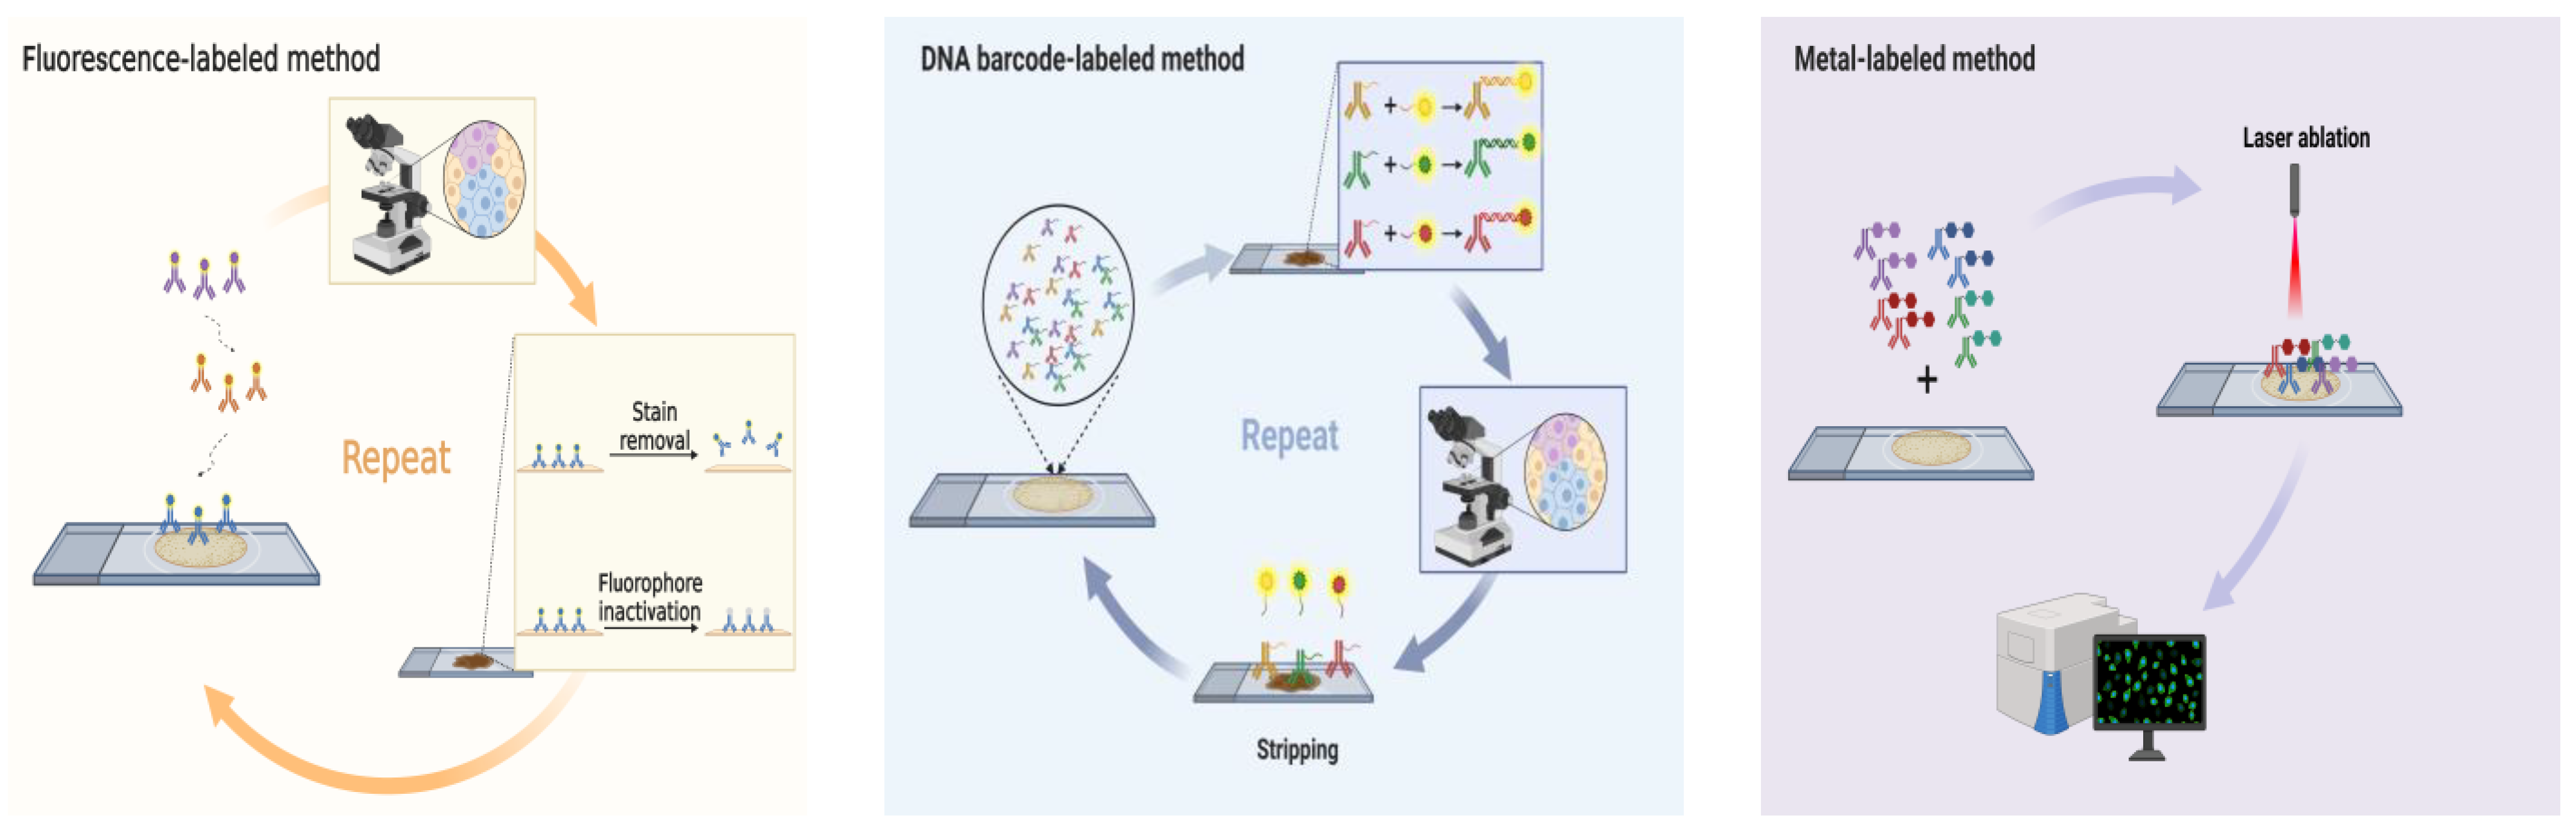
\includegraphics{mIFsteps.png}

}

\caption{\label{fig-1}Different methods for creating mIF/mIHC images.
Image courtesy of Sheng et al. (2023)}

\end{figure*}

mIHC/mIF images are widely used in studies for immune tumor
microenvironments (iTME). The studies often involves cell type
proportions within a certain region, spatial clustering of immune cells
or spatial interaction among different cell types (Wrobel, Harris, and
Vandekar 2023). For example: Schürch et al. (2020) discovered that
within granulcyte cell meightborhood, the enrichment PD-1+CD4+ T cells
are correlated with the survival outcome of a subset of colorectal
cancer patients; Chen et al. (2021) shows different immune cell
proportion and clustering between different colorectal tumor types;
Steinhart et al. (2021) found that certain immune cell proportions and
spatial interactions are correlated with ovarian cancer patient survival
outcomes.

\hypertarget{data-structure}{%
\section{Data Structure}\label{data-structure}}

For mIHC/mIF images, each individual ``plex'' corresponds to a different
immune protein identified by a type of stain. Each plex goes through
analogous transition as shown in Figure~\ref{fig-2} and form a table of
cell expressions, and the tables of different protein expressions are
combined in the end. Initially, greyscale intensity is assigned to each
pixel. The greyscale intensity is taken as the intensity of marker
expression. The image then goes through cell segmentation, which are
usually based on machine learning or deep learning methods(McKinley et
al. 2022; Schüffler et al. 2015). DAPI, a fluorescent stain typically
used for cell morphology identification, is most often used for the
initial cell segmentation. The same cell-segmentation will be used for
all other marker channels. Next, the pixel intensities, pixel positions,
and the cell that the pixel belongs to are entered into a dataframe.
Finally, the pixel intensities and position will be averaged within the
cell group. Often, the median of pixel intensities is used as well, to
reduce the impact of pixel intensity outliers. The end result after
combining all marker channels will be a dataset with each row
representing an individual cell, columns of different marker
expressions, and cell properties such as position, cell type (e.g.~tumor
cell or not, tissue type).

\begin{figure}

{\centering 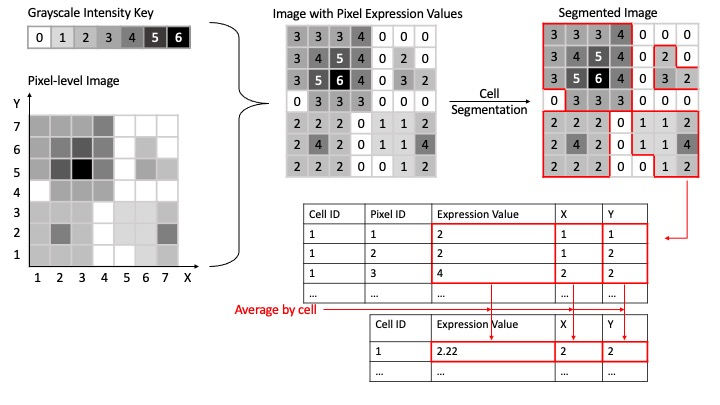
\includegraphics{mIFDataStr.jpg}

}

\caption{\label{fig-2}Transition from a single-plex mIHC/mIF image to a
single-cell dataframe. The greyscale intensity range is only a
demonstration. In application, the range of the greyscale intensity
depends on the configuration of image softwares. The cell intensity of
the bottom left cell is shown in the table as an example.}

\end{figure}

\bookmarksetup{startatroot}

\hypertarget{chapter-2-gammagater}{%
\chapter{Chapter 2: GammaGateR}\label{chapter-2-gammagater}}

\hypertarget{research-question}{%
\section{Research question}\label{research-question}}

Before important spatial insights can be gleaned using statistical
methods, mIF images undergo an intensive preprocessing pipeline to
obtain single-cell measurements. While there are various steps included
in the pipeline such as image registration, single-cell segmentation,
quantification, and batch correction, cell phenotyping is typically the
final step before downstream analyses on the cell-level data, similarly
to other single-cell assays. Cell phenotyping identifies individual cell
phenotypes from the measured marker expression values of the cell and
directly affects the subsequent cell population analysis results.

The two most common approaches for cell phenotyping in mIF are manual
gating and graph-based multivariate clustering. In manual gating, each
sample is visualized separately to determine a threshold, and
super-threshold cells are labeled as marker positive. This procedure is
repeated for all marker channels and slides, and the phenotypes are
determined by combining combinations of marker-positive cells.
Alternatively, multivariate graph-based clustering is adapted from other
single-cell assays. This approach first performs cell clustering, then
assigns a phenotype to each cell group based on their average expression
profile. Multivariate graph-based clustering is implemented with various
modifications across many software packages. Unfortunately, both methods
are labor intensive, and their accuracy suffers from image noise and
spatial artifacts in mIF images that cause marker expression histograms
to appear continuous or uni-modal . As a result, both phenotyping
methods possess shortcomings that cannot be ignored. On one hand, manual
gating can be subjective. On the other hand, graph-based clustering
results are prone to over-clustering and producing poor separation
between clusters.

\hypertarget{previous-works}{%
\section{Previous works}\label{previous-works}}

The challenges described above are well recognized and there are a few
methods and software developed that attempt to automate cell phenotyping
for mIF images. For example, CellSighter is a recently proposed
supervised deep-learning algorithm for cell phenotyping that requires a
``gold standard'' training dataset. Another recent solution, ASTIR
(Automated assignment of cell identity from single-cell multiplexed
imaging and proteomic data), is a fast unsupervised approach that
defines cell phenotypes from segmented cell-level data by using a neural
network-based mixture model assuming a multivariate log-normal
distribution. Instead of binary outputs like in classification methods,
ASTIR returns posterior probabilities of different cell types for each
cell. This type of output is advantageous because it offers more
information than nominal cell types and leaves cell labeling to the
clinician's discretion. Lastly, Ahmadian et al.~treat the analysis as a
pixel classification problem and design a single-step framework for mIF
phenotyping that is integrated with other preprocessing steps.

Nevertheless, inconsistencies persist in the results rendered by these
learning-based methods when applied across markers, slides, batches, and
datasets. These inconsistencies result from the immense variation in the
cell-level distribution of phenotyping markers that are often too
nuanced to be removed by existing batch correction methods. For these
reasons, it is difficult to fully automate the cell phenotyping process,
despite the availability of automated tools, and manual gating is still
used to perform cell phenotyping because it is easy to visualize and
evaluate the quality of the phenotype.

\hypertarget{methods}{%
\section{Methods}\label{methods}}

Because automated methods cannot be run without evaluation and
supervised methods require a gold-standard dataset, no method is truly
fully automated. As a solution, we develop an explicitly semi-automated
algorithm called GammaGateR. GammaGateR allows the user to easily
perform cell phenotyping, visualize results, and conduct interpretable
quality control while reducing manual labor. Based on a novel
closed-form Gamma mixture model (cfGMM), GammaGateR is a probabilistic
model that is fitted to each channel and slide separately, and outputs
positive-component probabilities for each marker. These can then be
easily thresholded and combined for semi-automated marker gating or
input directly into downstream analysis. GammaGateR has important
technical advantages, including 1) improved computation time and model
convergence due to its novel closed-form property, and 2) high
consistency and reproducibility for phenotyping results across mIF data
batches due to incorporation of parameter boundary constraints. In
applications on real-world mIF data, we find that GammaGateR has fast
and consistent results across many slides and markers. We provide an
open-source implementation of our method in the new GammaGateR R package
(https://github.com/jiangmeirubyxiong/gammagater).

\hypertarget{gammagater}{%
\subsection{GammaGateR}\label{gammagater}}

The GammaGateR algorithm is unique to existing methods for its focus on
parsimoniously modeling cell-level marker expression densities. This
approach yields tailored-to-slide model estimation in cell-level mIF
data where marker expression distributions can vary substantially across
slides. The algorithm uses a zero-inflated two-component GMM to model
marker expression for each slide. The Gamma mixture model naturally
identifies marker-positive and marker-negative cell distributions and
returns the probability of belonging to the marker-positive cell
distribution for each cell. The returned probabilities can either be
used directly in subsequent analysis or combined and dichotomized to
define cell phenotypes. GammaGateR incorporates user-specified
constraints to provide consistent model fit across a large number of
slides. The model evaluation methods included in GammaGateR allow the
user to evaluate the constraints and quality check results. The power
source of GammaGateR is the closed-form Gamma mixture model, which is a
novel approach to phenotyping for mIF data that makes it more
computationally efficient than traditional GMMs.

\begin{figure}

{\centering 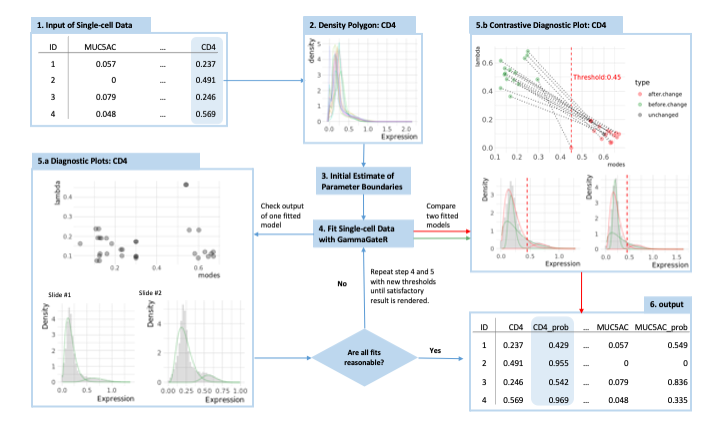
\includegraphics[width=1.2\textwidth,height=\textheight]{Figure1.png}

}

\caption{Figure 1}

\end{figure}

\hypertarget{cfgmm}{%
\subsection{cfGMM}\label{cfgmm}}

For mIF data, we use the GMM to fit cell marker expression values as a
weighted sum of different probability distributions that represent
unique cell populations {[}35{]}. The Gamma distribution is an excellent
model for marker values because the domain of the Gamma distribution is
strictly positive and it has the flexibility to model the varying skewed
densities seen in mIF marker values (Figure 1.5.a). However, GMMs are
not scalable for mIF image data, because they rely on computationally
inefficient numerical methods to obtain the maximum likelihood estimator
(MLE). The slow convergence of the MLE for the GMM makes it prohibitive
to apply across a large number of channels, slides, and cells. As a
solution, we develop a closed-form GMM (cfGMM;
https://github.com/jiangmeirubyxiong/cfgmm) estimation procedure based
on a recently developed estimator for the Gamma distribution {[}36{]}.
In addition, to improve computational efficiency, the cfGMM has the
benefit of allowing prior constraints on model parameters. With the
cfGMM in GammaGateR, we enable the flexibility to include a biologically
meaningful range for the mode of each component in the Gamma mixture
model. This way, users of GammaGateR can restrict estimation to
biologically meaningful values.

\hypertarget{derivation}{%
\subsubsection{Derivation}\label{derivation}}

We assume the data is a random sample \(x_1, \ldots, x_n\) from a \(K\)
component generalized gamma mixture distribution. The density function
of \(X\) is \begin{equation*}
P(X=x)=\sum_{k=1}^K \lambda_k f(x; a_k, b_k, \gamma_k).
\end{equation*} and the log-likelihood of the dataset is
\begin{equation}
    \ell(\mathbf{x}|\mathbf{a},\mathbf{b},\pmb{\lambda})=\sum^n_{i=1}\log\left\{\sum^K_{k=1}\lambda_kf(x_i|a_k,b_k)\right\}
    \label{eq:loglikelihood}
\end{equation} For each generalized gamma component \(k\),
\(\lambda_k\in [0,1]\) are the mixture parameters,
\(\sum_{k} \lambda_k = 1\); \(f\) denotes the generalized gamma density
function; \(a_k, b_k, \gamma_k\) are the parameters for the generalized
gamma.

Here, we use the expectation maximization (EM) algorithm
\citep{dempster_maximum_1977} for parameter estimation. EM algorithm is
a standard approach for parameter estimation in mixture models. It
introduces the latent multinomial variable
\(Z_{i} = (Z_{i1}, \ldots, Z_{iK})\) into the model and maximizes the
expected value of the complete data
likelihood\citep{dempster_maximum_1977}. The expectation of the complete
data likelihood to be maximized for the generalized gamma distribution
is \begin{equation*}
\mathbb{E}_Z \ell(x \mid Z) = \sum_{i=1}^n \sum_{k=1}^K z_{ik} \log f(x_i; a_k, b_k,\gamma_k),
\end{equation*} where \begin{equation}
 \label{eq:lambdaFormula}
    z_{ik} = \mathbb{P}(Z_{ik}=1 \mid x_i;\pmb{ a, b, \gamma} ) =\frac{f(x_i|a_k, b_k, \gamma_k)}{\displaystyle\sum^K_{j=1}f(x_i|a_j, b_j, \gamma_k)},
 \end{equation} \(\mathbf{a} = (a_1, a_2, \ldots, a_K)\), and
\(\mathbf{b}\), \(\pmb \lambda\) are similarly defined vectors.

From here, the maximization of the expectation is now analogous to the
maximization of generalized gamma distribution for each component of the
mixture model.

The expectation of log-likelihood is \begin{equation}
    \mathbb E_{z|x}[\log(L(\mathbf{x}|\mathbf{z}))]=\sum^{n}_{i=1}\sum^{K}_{k=1}z_{ik}\log f_k(x_i) \label{eq1}
\end{equation} and \begin{equation}
f_k(x)=G(a_k,b_k,{\gamma_k})=\frac{\lambda_k x^{a_k{\gamma_k}-1}exp\{(-x/b_k)^{{\gamma_k}}\}}{b_k^{a_k{\gamma_k}}\Gamma(a_k)} \label{eq2}
\end{equation} where \({\gamma_k}=1\).

By \eqref{eq1}, \eqref{eq2} The expected joint log-likelihood is
\begin{multline} \label{eq3}
     \mathbb E_{z|x}[\log(L(\mathbf{x}|\mathbf{z}))]=\sum^{K}_{k=1}\sum^{n}_{i=1}z_{ik}\left( \log{\gamma_k}-a_k{\gamma_k} \log b_k-log\Gamma(a_k)+(a_k{\gamma_k}-1)\log X_i-(\frac{X_i}{b_k})^{{\gamma_k}} \right)
\end{multline}

The estimators of each of the \(K\) terms of the expected joint
log-likelihood are derived as follows:

first take derivative of the expression from \eqref{eq3} \begin{align*}
    \sum^{n}_{i=1} z_{ik}\left( \log{\gamma_k}-a_k{\gamma_k} \log b_k-\log\Gamma(a_k)+(a_k{\gamma_k}-1)\log X_i-\left(\frac{X_i}{b_k}\right)^{\gamma_k} \right)
\end{align*} with respect to \(a_k, b_k, {\gamma_k}\) separately:\\
\begin{align}\label{eq4} 
      \frac{\partial \mathbb E_{z|x}[\log(L(\mathbf{x}|\mathbf{z}))]}{\partial a_k}
      =\sum^{n}_{i=1} z_{ik}(-\psi(a_k)-{\gamma_k} \log b_k+{\gamma_k} X_i)=0
  \end{align} Note that
\(\psi(x)=\displaystyle\frac{d }{dx}\log\Gamma(x)\) is digamma function.
\begin{align}\label{eq5} 
    \frac{\partial \mathbb E_{z|x}[\log(L(\mathbf{x}|\mathbf{z}))]}{\partial b_k}
    =\sum^{n}_{i=1}(z_{ik})(-a_k{\gamma_k}/b_k+{\gamma_k} X_i^{{\gamma_k}} b_k^{-{\gamma_k}-1})=0
\end{align} \begin{align}\label{eq6} 
    \frac{\partial \mathbb E_{z|x}[\log(L(\mathbf{x}|\mathbf{z}))]}{\partial {\gamma_k}}
    =\sum^{n}_{i=1}z_{ik}\left(\frac{1}{\gamma_k}-a_k\log b_k+a_k\log X_i-\left(\frac{X_i}{b_k}\right)^{\gamma_k} \log\frac{X_i}{b_k}\right)=0
\end{align} Among which, \eqref{eq5} can be solved as
\begin{equation} \label{eq7}
    \hat b_k(a_k,{\gamma_k})=\left(\frac{\displaystyle\sum^{n}_{i=1}z_{ik}X_i^{\gamma_k}}{a_k\displaystyle\sum^{n}_{i=1}z_{ik}}\right)^{1/{\gamma_k}}
\end{equation} Substitute \eqref{eq7} into \eqref{eq6}: \begin{align*}
    &\frac{\partial \mathbb E_{z|x}[\log(L(\mathbf{x}|\mathbf{z}))]}{\partial {\gamma_k}}\\
    &=\sum^{n}_{i=1}z_{ik}/{\gamma_k}+\sum^{n}_{i=1}a_kz_{ik}\log(\frac{X_i}{b_k})-\sum^{n}_{i=1}z_{ik}(\frac{X_i}{b_k}) ^{\gamma_k} \log(\frac{X_i}{b_k})\\
    &=\sum^{n}_{i=1}z_{ik}/{\gamma_k}+\sum^{n}_{i=1}a_kz_{ik}(\log X_i-\log b_k)-b_k^{-{\gamma_k}}\sum^{n}_{i=1}z_{ik}X_i ^{\gamma_k} (\log X_i-\log b_k)\\
    &=\sum^{n}_{i=1}z_{ik}/{\gamma_k}+\sum^{n}_{i=1}a_kz_{ik}\log X_i-\log b_k\sum^{n}_{i=1}a_kz_{ik}-b_k^{-{\gamma_k}}\sum^{n}_{i=1}z_{ik}X_i ^{\gamma_k} \log X_i+b_k^{-{\gamma_k}}\log b_k\sum^{n}_{i=1}z_{ik}X_i ^{\gamma_k}\\
    &=\sum^{n}_{i=1}z_{ik}/{\gamma_k}+\sum^{n}_{i=1}a_kz_{ik}\log X_i-\log b_k\sum^{n}_{i=1}a_kz_{ik}-b_k^{-{\gamma_k}}\sum^{n}_{i=1}z_{ik}X_i ^{\gamma_k} \log X_i
    \frac {a_k\displaystyle\sum^{n}_{i=1}z_{ik}}{\displaystyle\sum^{n}_{i=1}z_{ik}X_i^{\gamma_k}} \log b_k\displaystyle\sum^{n}_{i=1}z_{ik}X_i ^{\gamma_k}\\
    &=\sum^{n}_{i=1}z_{ik}/{\gamma_k}+\sum^{n}_{i=1}a_kz_{ik}\log X_i-\log b_k\sum^{n}_{i=1}a_kz_{ik}-b_k^{-{\gamma_k}}\sum^{n}_{i=1}z_{ik}X_i ^{\gamma_k} \log X_i+{a_k\sum^{n}_{i=1}z_{ik}}\log b_k\\
    &=\sum^{n}_{i=1}z_{ik}/{\gamma_k}+a_k\sum^{n}_{i=1}z_{ik}\log X_i-\frac {a_k\displaystyle\sum^{n}_{i=1}z_{ik}}{\displaystyle\sum^{n}_{i=1}z_{ik}X_i^{\gamma_k}}\sum^{n}_{i=1}z_{ik}X_i ^{\gamma_k} \log X_i\\
    &=\sum^{n}_{i=1}z_{ik}/{\gamma_k}+a_k\left(\sum^{n}_{i=1}z_{ik}\log X_i-\frac {\displaystyle\sum^{n}_{i=1}z_{ik}}{\displaystyle\sum^{n}_{i=1}z_{ik}X_i^{\gamma_k}}\sum^{n}_{i=1}z_{ik}X_i ^{\gamma_k} \log X_i\right)=0\\
\end{align*}\\
Solving this, we have \begin{equation} \label{eq8}
      \hat a_k ({\gamma_k})=\displaystyle\frac{\displaystyle\sum^{n}_{i=1}\displaystyle\frac{z_{ik}}{{\gamma_k}}}
      {\displaystyle\frac{\displaystyle\sum^{n}_{i=1}z_{ik}}{\displaystyle\sum^{n}_{i=1}z_{ik}X_i^{\gamma_k}}\sum^{n}_{i=1}z_{ik}X_i ^{\gamma_k} \log X_i-\sum^{n}_{i=1}z_{ik}\log X_i}
  \end{equation}

Plug \({\gamma_k}=1\) in \eqref{eq8}, we now have \begin{align}
  \hat a_k ({\gamma_k}=1)&=\displaystyle\frac{\displaystyle\sum^{n}_{i=1}z_{ik}}{\displaystyle\frac {\displaystyle\sum^{n}_{i=1}z_{ik}}{\displaystyle\sum^{n}_{i=1}z_{ik}X_i}\sum^{n}_{i=1}z_{ik}X_i  \log X_i-\sum^{n}_{i=1}z_{ik}\log X_i}\nonumber\\
  &=\left(\frac {\sum^{n}_{i=1}z_{ik}X_i\log X_i}{\sum^{n}_{i=1}z_{ik}X_i}-\frac{\sum^{n}_{i=1}z_{ik}\log X_i}{\sum^{n}_{i=1}z_{ik}}\right)^{-1}\nonumber\\
  &=\frac{\displaystyle\sum^{n}_{i=1}z_{ik}\displaystyle\sum^{n}_{i=1}z_{ik}X_i}{\displaystyle\sum^{n}_{i=1}z_{ik}\displaystyle\sum^{n}_{i=1}z_{ik}X_i\log X_i-\displaystyle\sum^{n}_{i=1}z_{ik}\log X_i\displaystyle\sum^{n}_{i=1}z_{ik}X_i}\label{eq:ak}
  \end{align} \begin{align}
        \hat b_k(\hat a_k,{\gamma_k}=1)&=\frac{\displaystyle\sum^{n}_{i=1}z_{ik}X_i}{\hat a_k\displaystyle\sum^{n}_{i=1}z_{ik}} \nonumber\\
        %&=\displaystyle\frac{\displaystyle\sum^{n}_{i=1}z_{ik}X_i}{\displaystyle\frac{\displaystyle\sum^{n}_{i=1}z_{ik}X_i\displaystyle\sum^{n}_{i=1}z_{ik}}{\displaystyle\sum^{n}_{i=1}z_{ik}\displaystyle\sum^{n}_{i=1}z_{ik}X_i\log X_i-\displaystyle\sum^{n}_{i=1}z_{ik}\log X_i\displaystyle\sum^{n}_{i=1}z_{ik}X_i}\displaystyle\sum^{n}_{i=1}z_{ik}} \nonumber\\
        &=\frac{\displaystyle\sum^{n}_{i=1}z_{ik}\displaystyle\sum^{n}_{i=1}z_{ik}X_i\log X_i-\displaystyle\sum^{n}_{i=1}z_{ik}\log X_i\displaystyle\sum^{n}_{i=1}z_{ik}X_i}{\left(\displaystyle\sum^{n}_{i=1}z_{ik}\right)^2} \label{eq:bk}
  \end{align} In addition, \(\hat {\lambda}_k\) can simply be estimated
as \begin{equation}
    \hat {\lambda}_k =\frac{\displaystyle\sum^{n}_{i=1}z_{ik}}{n} \label{eq:lambdak}
 \end{equation}

It is worth noting that we are not maximizing the exact Gamma
distribution, therefore the algorithm we devise here is an EM-type
algorithm.

\hypertarget{simulation}{%
\section{Simulation}\label{simulation}}

\begin{marginfigure}

{\centering 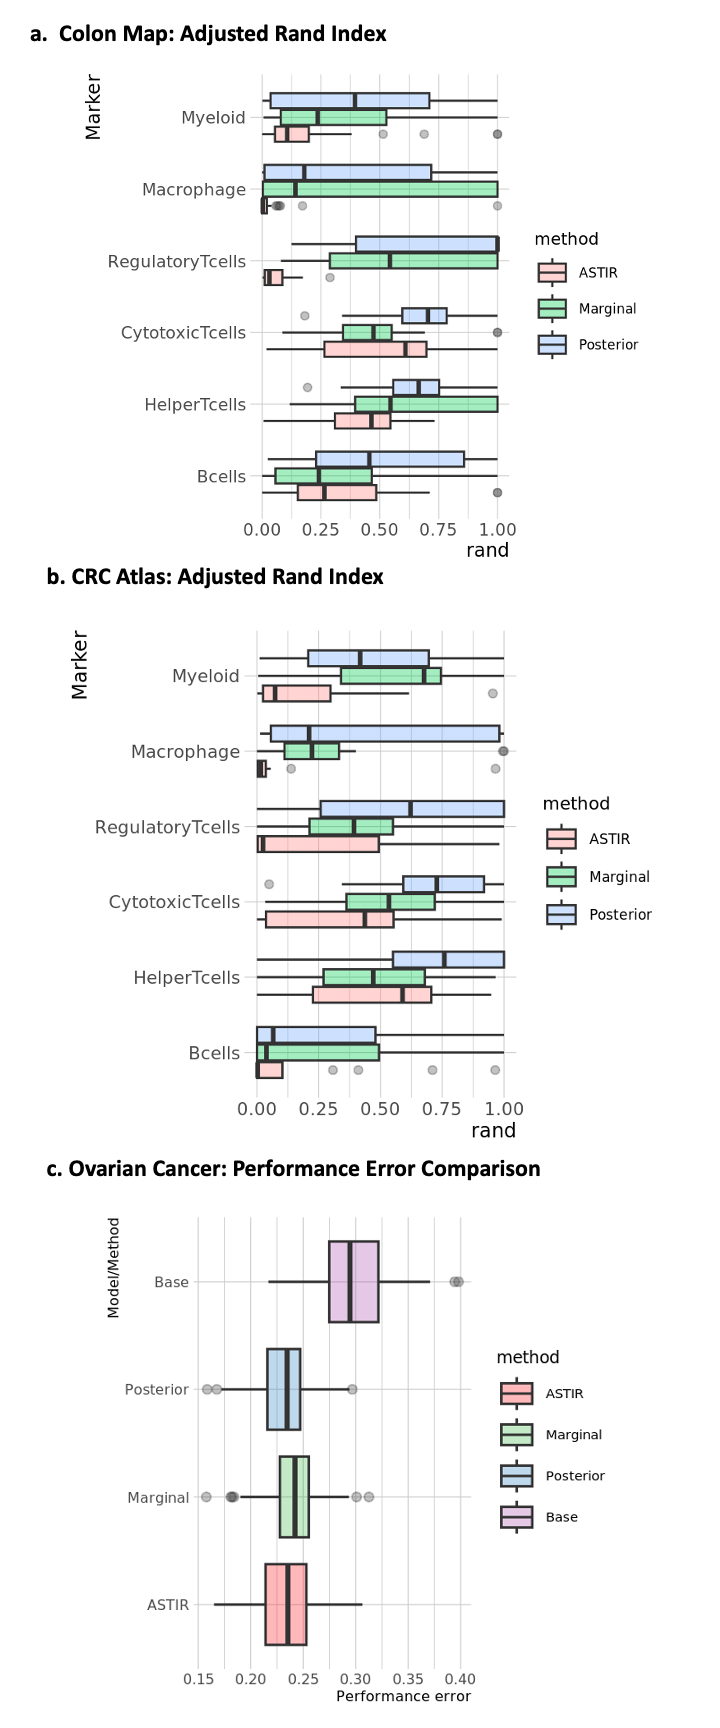
\includegraphics{Figure2.png}

}

\caption{Figure 2}

\end{marginfigure}

To compare the bias and compute time of the closed-form GMM to maximum
likelihood GMM implementation, we run the cfGMM, the constrained cfGMM,
and the GMM to evaluate bias and variance in a sample size of 10,000
across 1,000 simulations. We simulate a two-component mixture model with
parameters
\(\pmb{\lambda} = (0.3, 0.7), \pmb{a} = (0.5, 8), \pmb{b} = (0.5, 1/3)\).
For the constrained estimator, we restrict the mode of each component to
be in the range \((-\infty, 0)\) and \((0,5)\) for marker negative and
marker positive components, respectively, which include the true mode
for each component, \(0\) (no mode) and \(7/3\).

Both closed-form estimation procedures have substantially faster
computation time than the MLE (Figure 2a) while maintaining similarly
low bias (Figure 2b). The sample size used in the simulation is roughly
similar to that of the cell-level mIF image dataset, which further
proves that cfGMM brings computation efficiency to our target
application. The closed-form GMM, therefore, enables computationally
feasible, precise, and flexible model estimation when applied to a large
number of channels and slides using GammaGateR. It is also worth noting
that the constrained cfGMM converges slightly faster than without
constraints. This implies that when using cfGMM, computational cost can
be reduced with proper knowledge of biological priors.

\hypertarget{analysis}{%
\section{Analysis}\label{analysis}}

\bookmarksetup{startatroot}

\hypertarget{sec-imputation}{%
\chapter{Chapter 3: Missing data imputation in mIF
imaging}\label{sec-imputation}}

Just like all data created and collected by human being, missing data is
inevitable in mIF image as well. Bao et al. (2021) in their paper gave a
brief summary of types of missing data in mIF image, as in
Figure~\ref{fig-31}. Case 1 in Figure~\ref{fig-31} refers to the missing
of one or more entire marker channel. This type of missing data occurs
but rarely, often due to low image quality. Another possible reason for
missing channel, not described in Bao et al. (2021), can be supply
shortage in certain type of fluorescent material or change in research
plan. Despite the rarity of case 1, there are demand for marker channel
imputation with low-plex images. Due to time and financial constraints,
mIF with no more than seven channels are often more feasible to obtain
than the 40-channel mIFs(Wu et al. 2023). To break the restraint in
obtaining cell phenotypes from few number of markers, imputation of
marker channels are proposed. Case 2 Figure~\ref{fig-31} occurs more
frequently, when tissue wears off in the cycles of staining - wash off
described in Figure~\ref{fig-1}.

Owning to the rapid development in the field of computer vision, all
current applications in mIF imputation are implemented with machine
learning and/or deep learning methods. In the three applications covered
in this document today, Bao et al. (2021) uses generative adversarial
networks (GANs), Wu et al. (2023) uses gradient boosting decision tree
in combination with convolutional neural network, and Sims and Chang
(2023) uses variational autoencoders (VAE). All methods preforms ideally
well, as expected out of the maturity of machine learning methods.
However, the subsequent analysis can benefit from statistical thinking
in data imputation. This will be discussed further in chapter 4.

\begin{figure}

{\centering 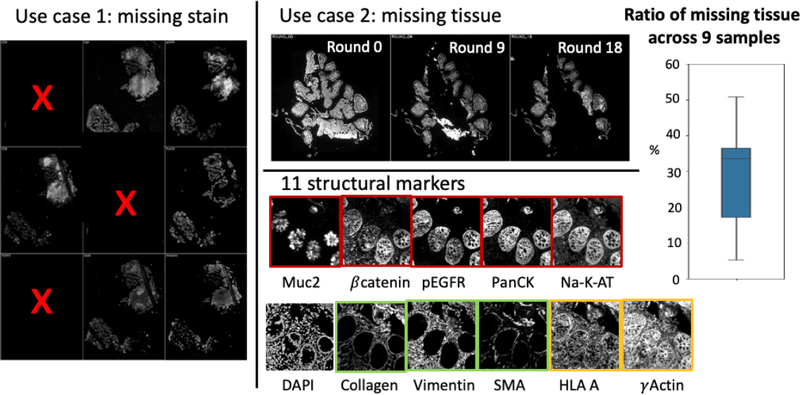
\includegraphics{missingmIF.jpeg}

}

\caption{\label{fig-31}Types of missing data in mIF. Image courtesy of
Bao et al. (2021).}

\end{figure}

\hypertarget{application-case-1-missing-tissue-imputation}{%
\section{Application case 1: Missing tissue
imputation}\label{application-case-1-missing-tissue-imputation}}

\hypertarget{method-gan}{%
\subsection{Method: GAN}\label{method-gan}}

\hypertarget{sec-imputation1}{%
\subsection{Application in mIF: pix2pixHD}\label{sec-imputation1}}

\hypertarget{application-case-2-marker-channel-imputation}{%
\section{Application case 2: marker channel
imputation}\label{application-case-2-marker-channel-imputation}}

\hypertarget{sec-imputation2}{%
\subsection{Application 2.1: 7-UP}\label{sec-imputation2}}

\hypertarget{sec-imputation3}{%
\subsection{Application 2.2: CyCIF panel
reduction}\label{sec-imputation3}}

\bookmarksetup{startatroot}

\hypertarget{chapter-4-future-directions}{%
\chapter{Chapter 4: future
directions}\label{chapter-4-future-directions}}

The missing data in mIF image can be see as missing completely at random
(MCAR). In the missing data scenarios described in
(\textbf{section-imputation?}), the missingness cannot be predicted in
any of the scenario. However, for low-plex image channel imputation, the
markers are selected by machine learning methods to maximize the
accuracy. For this type of imputation, the imputation results should be
taken with a grain of salt as this is missing not at random (MNAR). It
might be possible to deduct the amount of bias this creates through
statistical inference, but for now this is not in the scope of this
project.

All methods in Chapter~\ref{sec-imputation} evaluated the accuracy of
their result by either comparing with the imputation outcome of a
previous method or with a held-out evaluation dataset. In addition, Wu
et al. (2023) in Section~\ref{sec-imputation2} used the imputation
output for cell phenotyping and predicting patient phenotypic outcomes.
In principle, this is not the best practice of subsequent analysis with
the imputation outcome. Such prediction should be performed with
multiple imputation at least, to obtain a better estimation of
confidence intervals.

\bookmarksetup{startatroot}

\hypertarget{references}{%
\chapter*{References}\label{references}}
\addcontentsline{toc}{chapter}{References}

\markboth{References}{References}

\hypertarget{refs}{}
\begin{CSLReferences}{1}{0}
\leavevmode\vadjust pre{\hypertarget{ref-bao2021random}{}}%
Bao, Shunxing, Yucheng Tang, Ho Hin Lee, Riqiang Gao, Sophie Chiron,
Ilwoo Lyu, Lori A Coburn, et al. 2021. {``Random Multi-Channel Image
Synthesis for Multiplexed Immunofluorescence Imaging.''} In \emph{MICCAI
Workshop on Computational Pathology}, 36--46. PMLR.

\leavevmode\vadjust pre{\hypertarget{ref-chen2021differential}{}}%
Chen, Bob, Scurrah Cherie'R, Eliot T McKinley, Alan J Simmons, Marisol A
Ramirez-Solano, Xiangzhu Zhu, Nicholas O Markham, et al. 2021.
{``Differential Pre-Malignant Programs and Microenvironment Chart
Distinct Paths to Malignancy in Human Colorectal Polyps.''} \emph{Cell}
184 (26): 6262--80.

\leavevmode\vadjust pre{\hypertarget{ref-coons1941immunological}{}}%
Coons, Albert H, Hugh J Creech, and R Norman Jones. 1941.
{``Immunological Properties of an Antibody Containing a Fluorescent
Group.''} \emph{Proceedings of the Society for Experimental Biology and
Medicine} 47 (2): 200--202.

\leavevmode\vadjust pre{\hypertarget{ref-duraiyan2012applications}{}}%
Duraiyan, Jeyapradha, Rajeshwar Govindarajan, Karunakaran Kaliyappan,
and Murugesan Palanisamy. 2012. {``Applications of
Immunohistochemistry.''} \emph{Journal of Pharmacy \& Bioallied
Sciences} 4 (Suppl 2): S307.

\leavevmode\vadjust pre{\hypertarget{ref-eng2022framework}{}}%
Eng, Jennifer, Elmar Bucher, Zhi Hu, Ting Zheng, Summer L Gibbs, Koei
Chin, and Joe W Gray. 2022. {``A Framework for Multiplex Imaging
Optimization and Reproducible Analysis.''} \emph{Communications Biology}
5 (1): 438.

\leavevmode\vadjust pre{\hypertarget{ref-hussaini2022immunohistochemistry}{}}%
Hussaini, Haizal Mohd, Benedict Seo, and Alison M Rich. 2022.
{``Immunohistochemistry and Immunofluorescence.''} In \emph{Oral
Biology: Molecular Techniques and Applications}, 439--50. Springer.

\leavevmode\vadjust pre{\hypertarget{ref-mckinley2022miriam}{}}%
McKinley, Eliot T, Justin Shao, Samuel T Ellis, Cody N Heiser, Joseph T
Roland, Mary C Macedonia, Paige N Vega, Susie Shin, Robert J Coffey, and
Ken S Lau. 2022. {``MIRIAM: A Machine and Deep Learning Single-Cell
Segmentation and Quantification Pipeline for Multi-Dimensional Tissue
Images.''} \emph{Cytometry Part A} 101 (6): 521--28.

\leavevmode\vadjust pre{\hypertarget{ref-ramos2005technical}{}}%
Ramos-Vara, Jose A. 2005. {``Technical Aspects of
Immunohistochemistry.''} \emph{Veterinary Pathology} 42 (4): 405--26.

\leavevmode\vadjust pre{\hypertarget{ref-schuffler2015automatic}{}}%
Schüffler, Peter J, Denis Schapiro, Charlotte Giesen, Hao AO Wang, Bernd
Bodenmiller, and Joachim M Buhmann. 2015. {``Automatic Single Cell
Segmentation on Highly Multiplexed Tissue Images.''} \emph{Cytometry
Part A} 87 (10): 936--42.

\leavevmode\vadjust pre{\hypertarget{ref-schurch2020coordinated}{}}%
Schürch, Christian M, Salil S Bhate, Graham L Barlow, Darci J Phillips,
Luca Noti, Inti Zlobec, Pauline Chu, et al. 2020. {``Coordinated
Cellular Neighborhoods Orchestrate Antitumoral Immunity at the
Colorectal Cancer Invasive Front.''} \emph{Cell} 182 (5): 1341--59.

\leavevmode\vadjust pre{\hypertarget{ref-sheng2023multiplex}{}}%
Sheng, Wenjie, Chaoyu Zhang, TM Mohiuddin, Marwah Al-Rawe, Felix
Zeppernick, Franco H Falcone, Ivo Meinhold-Heerlein, and Ahmad Fawzi
Hussain. 2023. {``Multiplex Immunofluorescence: A Powerful Tool in
Cancer Immunotherapy.''} \emph{International Journal of Molecular
Sciences} 24 (4): 3086.

\leavevmode\vadjust pre{\hypertarget{ref-sims2023masked}{}}%
Sims, Zachary, and Young Hwan Chang. 2023. {``A Masked Image Modeling
Approach to Cyclic Immunofluorescence (CyCIF) Panel Reduction and Marker
Imputation.''} \emph{bioRxiv}, 2023--05.

\leavevmode\vadjust pre{\hypertarget{ref-steinhart2021spatial}{}}%
Steinhart, Benjamin, Kimberly R Jordan, Jaidev Bapat, Miriam D Post,
Lindsay W Brubaker, Benjamin G Bitler, and Julia Wrobel. 2021. {``The
Spatial Context of Tumor-Infiltrating Immune Cells Associates with
Improved Ovarian Cancer Survival.''} \emph{Molecular Cancer Research} 19
(12): 1973--79.

\leavevmode\vadjust pre{\hypertarget{ref-wrobel2023statistical}{}}%
Wrobel, Julia, Coleman Harris, and Simon Vandekar. 2023. {``Statistical
Analysis of Multiplex Immunofluorescence and Immunohistochemistry
Imaging Data.''} In \emph{Statistical Genomics}, 141--68. Springer.

\leavevmode\vadjust pre{\hypertarget{ref-wu20237}{}}%
Wu, Eric, Alexandro E Trevino, Zhenqin Wu, Kyle Swanson, Honesty J Kim,
H Blaize D'Angio, Ryan Preska, et al. 2023. {``7-UP: Generating in
Silico CODEX from a Small Set of Immunofluorescence Markers.''}
\emph{PNAS Nexus} 2 (6): pgad171.

\end{CSLReferences}



\end{document}
